% !TEX program = lualatex
\documentclass[10pt,aspectratio=169]{beamer}

% Reduce "Overfull \\vbox" warnings in beamer
\raggedbottom
% Suppress tiny overfull box warnings (layout is fine)
\hfuzz=3pt
\vfuzz=10pt
\setlength{\emergencystretch}{3em}

% Use ctex; we set CJK fonts explicitly below to avoid missing Japanese glyphs
\usepackage[fontset=none]{ctex}
\usepackage{hyperref}
\usepackage{tikz}
\usetikzlibrary{decorations.pathreplacing,shadows}

% CJK main font
\IfFontExistsTF{Noto Serif CJK JP}{
  \setCJKmainfont{Noto Serif CJK JP}
}{
  \IfFontExistsTF{HaranoAjiMincho-Regular}{
    \setCJKmainfont{HaranoAjiMincho-Regular}
  }{
    \IfFontExistsTF{HaranoAjiMincho}{
      \setCJKmainfont{HaranoAjiMincho}
    }{
      \IfFontExistsTF{IPAexMincho}{
        \setCJKmainfont{IPAexMincho}
      }{
        \IfFontExistsTF{FandolSong-Regular}{
          \setCJKmainfont{FandolSong-Regular}
        }{}
      }
    }
  }
}

% CJK sans font
\IfFontExistsTF{HaranoAjiGothic-Medium}{
  \IfFontExistsTF{HaranoAjiGothic-Bold}{
    \setCJKsansfont[BoldFont=HaranoAjiGothic-Bold]{HaranoAjiGothic-Medium}
  }{
    \setCJKsansfont[BoldFont=HaranoAjiGothic-Medium,BoldFeatures={FakeBold=2}]{HaranoAjiGothic-Medium}
  }
}{
  \IfFontExistsTF{HaranoAjiGothic}{
    \setCJKsansfont[BoldFont=HaranoAjiGothic,BoldFeatures={FakeBold=2}]{HaranoAjiGothic}
  }{
    \IfFontExistsTF{Noto Sans CJK JP}{
      \setCJKsansfont{Noto Sans CJK JP}
    }{
      \IfFontExistsTF{IPAexGothic}{
        \setCJKsansfont{IPAexGothic}
      }{
        \IfFontExistsTF{FandolHei-Regular}{
          \setCJKsansfont{FandolHei-Regular}
        }{}
      }
    }
  }
}
\IfFontExistsTF{HaranoAjiGothic-Medium}{
  \setCJKmonofont{HaranoAjiGothic-Medium}
}{
  \IfFontExistsTF{Noto Sans Mono CJK JP}{
    \setCJKmonofont{Noto Sans Mono CJK JP}
  }{}
}

% Japanese font family
\IfFontExistsTF{Noto Serif CJK JP}{
  \newCJKfontfamily\jp{Noto Serif CJK JP}
}{
  \IfFontExistsTF{HaranoAjiMincho-Regular}{
    \newCJKfontfamily\jp{HaranoAjiMincho-Regular}
  }{
    \IfFontExistsTF{HaranoAjiMincho}{
      \newCJKfontfamily\jp{HaranoAjiMincho}
    }{
      \IfFontExistsTF{IPAexMincho}{
        \newCJKfontfamily\jp{IPAexMincho}
      }{
        \newcommand{\jp}{}
      }
    }
  }
}

% other packages
\usepackage{latexsym,amsmath,multicol,booktabs,calligra}
\usepackage{array}
\usepackage[table]{xcolor}
\usepackage{graphicx,listings,stackengine}
\usepackage{tikz}
\usetikzlibrary{arrows.meta,positioning,calc}

\author{王童語}
\title{Tadasunomori試作UI開発}
\subtitle{AI活用によるC++実装とVM環境での検証}
\institute{研究開発本部\\大阪開発センター}
\date{2026年2月10日}
\usepackage{Arkray}

% ★修正: titlegraphic を1回だけ定義（重複削除）
\titlegraphic{\includegraphics[height=1.0cm]{pic/Arkray\space brand\space logo.png}}

\begin{document}

\begin{frame}
  \titlepage
  \vspace{1em}
  \centering
  {\tiny Generated by Cursor Agent (Models: Cursor Auto Mode) and Debug with OpenAI Prism}
\end{frame}

\section{Overview}
\begin{frame}[t]{今日の話の概要}

  % ★修正: 「GUIが搭載する」→「GUIを搭載する」
  \begin{block}{プロジェクト背景：Tadasunomori試作UIの作成}
    \begin{itemize}
      \item 一次試作機にGUIを搭載することを目指して
        \begin{itemize}
        \item 一次試作機が完成する時点で、試作機の操作をCLI形式でなく、GUI形式で表示すること
      \end{itemize}
    \end{itemize}
  \end{block}

  % ★修正: 「快速的開発」→「迅速な開発」
  \begin{block}{プロジェクト遂行：End-to-Endの方法で迅速な開発}
  \vspace{0.5em}
    \centering
    \begin{tikzpicture}[
        node distance=1.4cm,
        box/.style={rounded corners,align=center,inner sep=4pt,
                    text width=0.42\linewidth,minimum height=1.2cm,
                    line width=0.8pt},
        arr/.style={-{Stealth[length=3mm,width=2mm]},very thick,color=red!70!black}
      ]
      \node[box,draw=orange!60!black,fill=orange!10,
            drop shadow={shadow xshift=0.5pt,shadow yshift=-0.5pt,fill=black!15}]
        (old) {\textbf{従来（人手中心）}\\[-0.4em]
          {\scriptsize 人間で設計\,$\rightarrow$\,実装\,$\rightarrow$\,検証（サイクル）}
        };
      \node[box,draw=tsinghua!80,fill=tsinghua!10,
            drop shadow={shadow xshift=0.5pt,shadow yshift=-0.5pt,fill=black!15},
            right=of old]
        (new) {\textbf{新方式（AIエージェント活用）}\\[-0.4em]
          {\scriptsize Cursor・Copilot多Agent\,$\rightarrow$\,開発実装\,$\rightarrow$\,検証とDebug}
        };
      \draw[arr] (old) -- (new);
    \end{tikzpicture}
  \end{block}


  % ★修正: 「相応し」→「対応する」、「低資源消耗」→「低リソース消費」、「周り」→「周辺」
  \begin{block}{プロジェクト成果：三つの測定フローに対応する操作画面の実現}
    \begin{itemize}
      \item $C\!+\!+17$に基づいた組み込み向け低リソース消費GUIをLinux環境で実装
      \begin{itemize}
        \item 現段階で全測定フローが完成、周辺機能（機械設定やメンテナンスモードなど）は未搭載
      \end{itemize}
    \end{itemize}
  \end{block}

\end{frame}

% ★修正: 「プロジェクと概要」→「プロジェクト概要」
\section{プロジェクト概要}
\begin{frame}[t]{プロジェクト概要：Cursor主導の開発アプローチ}
  \small
  \begin{block}{計画から実装までの一貫したサポート}
    AIエージェント「Cursor」を活用し、設計・環境構築・実装・デバッグの全工程を効率化。
  \end{block}

  \begin{center}
    
\includegraphics[width=\linewidth,height=2.4cm,keepaspectratio]{pic/9-1.png}
  \end{center}

  \vspace{-2em}
  \begin{columns}[T,onlytextwidth]
    \begin{column}{0.48\textwidth}
      \begin{block}{ターゲット環境}
        \begin{itemize}\setlength\itemsep{0.25em}
          \item \textbf{環境:} VMware Workstation上のUbuntu VM
          \item \textbf{言語:} $C\!+\!+17$（堅牢性・メモリ安全性）
          % ★修正: 末尾の「!」を削除
          \item \textbf{GUI:} LVGL 9.2（組み込み向け軽量GUI）
        \end{itemize}
      \end{block}
    \end{column}
    \begin{column}{0.48\textwidth}
      \begin{block}{Cursorの役割}
        \begin{itemize}\setlength\itemsep{0.25em}
          \item \textbf{インフラ:} 複雑なSSH接続手順の自動生成
          \item \textbf{移行:} ReactプロトタイプからC++への翻訳
          \item \textbf{品質:} 対話的なレイアウト調整とバグ修正
        \end{itemize}
      \end{block}
    \end{column}
  \end{columns}
\end{frame}

\section{フェーズ1}
\begin{frame}[t]{フェーズ1：インフラ構築（VM接続）}
  \small
  \begin{block}{VMware NAT環境へのアクセス課題}
    \textbf{課題:} ホストPC（Jig PC）上のNAT環境にあるUbuntu VMへ、開発用PC（Cyber PC）から直接SSH接続できない。
  \end{block}

  \vspace{0.3em}
  \centering
  \begin{tikzpicture}[
      node/.style={rounded corners,minimum width=0.23\linewidth,
                   minimum height=1.15cm,align=center,line width=0.8pt},
      arr/.style={-Latex,thick},
      lbl/.style={font=\scriptsize,fill=white,inner sep=2pt,rounded corners=2pt}
    ]
    \node[node,draw=blue!50,fill=blue!8,
          drop shadow={shadow xshift=0.5pt,shadow yshift=-0.5pt,fill=black!12}]
      (cy) {\textbf{Cyber PC}\\開発者端末};
    \node[node,draw=orange!50,fill=orange!10,
          drop shadow={shadow xshift=0.5pt,shadow yshift=-0.5pt,fill=black!12},
          right=2.0cm of cy]
      (jig) {\textbf{Jig PC (Windows)}\\169.254.57.112};
    \node[node,draw=tsinghua!60,fill=tsinghua!10,
          drop shadow={shadow xshift=0.5pt,shadow yshift=-0.5pt,fill=black!12},
          right=2.0cm of jig]
      (vm) {\textbf{Ubuntu VM}\\192.168.247.128};

    \draw[arr,color=blue!60!black] (cy) -- node[lbl,above,yshift=1pt]{SSH\;Port 2222} (jig);
    \draw[arr,color=tsinghua!80] (jig) -- node[lbl,above,yshift=1pt]{PortProxy (NAT)} (vm);
  \end{tikzpicture}


  \vspace{0.4em}
  \begin{columns}[T,onlytextwidth]
    \begin{column}{0.48\textwidth}
      \begin{block}{解決策：Windows PortProxy}
        Cursorがネットワーク構造を分析し、中継地点であるJig PCにポート転送ルールを設定。
      \end{block}
    \end{column}
    \begin{column}{0.48\textwidth}
      \begin{block}{デバッグ結果}
        当初の「接続タイムアウト」エラーに対し、ファイアウォール設定の不備を指摘し解決。
      \end{block}
    \end{column}
  \end{columns}
\end{frame}

\section{フェーズ1.5}
\begin{frame}[t,fragile]{フェーズ1.5：ビルドとデプロイメントの自動化}
  \small
  \begin{block}{オフライン環境下での双方向開発フロー}
    インターネット接続のないJig PCへのデプロイとリモート操作を確立。
  \end{block}

  \vspace{0.3em}
  \centering
  \begin{tikzpicture}[
      box/.style={rounded corners,minimum width=0.24\linewidth,
                  minimum height=1.4cm,align=center,line width=0.8pt},
      arr/.style={-Latex,thick},
      lbl/.style={font=\scriptsize,fill=white,inner sep=2pt,rounded corners=2pt}
    ]
    \node[box,draw=blue!40,fill=blue!8,
          drop shadow={shadow xshift=0.5pt,shadow yshift=-0.5pt,fill=black!12}]
      (w) {\textbf{Windows (Local)}\\Cursor Agent};
    \node[box,draw=tsinghua!60,fill=tsinghua!10,
          drop shadow={shadow xshift=0.5pt,shadow yshift=-0.5pt,fill=black!12},
          right=2.4cm of w]
      (u) {\textbf{Ubuntu (VM)}\\ビルド・実行};
    \draw[arr,color=tsinghua!70!black]
      ([yshift=7pt]w.east) -- node[lbl,above,yshift=4pt]{RDP / SSH} ([yshift=7pt]u.west);
    \draw[arr,color=red!60]
      ([yshift=-7pt]w.east) -- node[lbl,below,yshift=-1pt]{SCP (Upload)} ([yshift=-7pt]u.west);
    \draw[arr,color=green!60!black]
      ([yshift=-7pt]u.west) -- node[lbl,below,yshift=-9pt]{SCP (Download)} ([yshift=-7pt]w.east);
  \end{tikzpicture}


  \vspace{-1em}
  \begin{columns}[T,onlytextwidth]
    \begin{column}{0.48\textwidth}
      \begin{block}{主なツール}
        \begin{itemize}\setlength\itemsep{0.25em}
          \item \textbf{MSTSC (RDP):}
          \begin{lstlisting}[numbers=none,frame=single]
          mstsc /v:169.254.57.112
          \end{lstlisting}
          \item \textbf{PowerShell:} 自動生成スクリプトによるファイル転送
        \end{itemize}
      \end{block}
    \end{column}
    \begin{column}{0.48\textwidth}
      \begin{block}{双方向の同期}
        \begin{itemize}\setlength\itemsep{0.25em}
          \item \textbf{Upload:} ソースコードの更新を即時反映
          \item \textbf{Download:} VM上で生成されたログやデータを回収
        \end{itemize}
      \end{block}
    \end{column}
  \end{columns}
\end{frame}

\section{フェーズ2}
\begin{frame}[t]{フェーズ2：ReactからC++への移行戦略（プロセス）}
  \small
  \begin{block}{Webの柔軟性を組み込みの堅牢性へ}
    プロトタイプから最終製品まで、Cursorが各フェーズで専門的な役割を果たす。
  \end{block}

  \vspace{2.2em}
  \centering
  \begin{tikzpicture}[scale=0.88,transform shape,
      proc/.style={rounded corners,minimum width=0.29\linewidth,
                   minimum height=2.6cm,align=left,inner sep=6pt,
                   line width=0.8pt},
      arr/.style={-Latex,very thick},
      num/.style={circle,font=\small\bfseries,text=white,
                  minimum size=0.45cm,inner sep=0pt}
    ]
    \node[proc,draw=orange!50,fill=orange!8,
          drop shadow={shadow xshift=0.6pt,shadow yshift=-0.6pt,fill=black!12}]
      (a) {%
        \textbf{1. プロトタイプ生成}\\[1em]
        \footnotesize
        \begin{tabular}{@{}l@{}}
          \textbullet\;\textbf{Figma}\\（UIフローチャート設計）\\[0.7em]
          \textbullet\;\textbf{Figma Make}\\（AIによるコード化）\\[0.7em]
          \textbullet\;\textbf{React App}\\（動作確認用UI）
        \end{tabular}
      };
    \node[proc,draw=yellow!60!black,fill=yellow!10,
          drop shadow={shadow xshift=0.6pt,shadow yshift=-0.6pt,fill=black!12},
          right=1cm of a]
      (b) {%
        \textbf{2. AIによる移行（Cursor）}\\[1em]
        \footnotesize
        \begin{tabular}{@{}l@{}}
          \textbullet\;\textbf{Code Analysis}\\（React構造の解析）\\[0.7em]
          \textbullet\;\textbf{Plan Mode}\\（C++クラス設計・計画）\\[0.7em]
          \textbullet\;\textbf{Agent Implementation}\\（LVGLコード生成）
        \end{tabular}
      };
    \node[proc,draw=tsinghua!60,fill=tsinghua!10,
          drop shadow={shadow xshift=0.6pt,shadow yshift=-0.6pt,fill=black!12},
          right=1cm of b]
      (c) {%
        \textbf{3. 実装と検証}\\[1em]
        \footnotesize
        \begin{tabular}{@{}l@{}}
          \textbullet\;\textbf{C++ / LVGL}\\（ターゲットコード）\\[0.7em]
          \textbullet\;\textbf{Verifying}\\（実装環境で動作確認）\\[0.7em]
          \textbullet\;\textbf{Debug / Fix}\\（実機動作検証）
        \end{tabular}
      };

    \draw[arr,color=orange!70!black] (a) -- (b);
    \draw[arr,color=tsinghua!70!black] (b) -- (c);

    % フェーズ番号の円形バッジ
    \node[num,fill=orange!70!black] at ([xshift=-0.15cm,yshift=0.15cm]a.north west) {1};
    \node[num,fill=yellow!60!black] at ([xshift=-0.15cm,yshift=0.15cm]b.north west) {2};
    \node[num,fill=tsinghua!80]     at ([xshift=-0.15cm,yshift=0.15cm]c.north west) {3};
  \end{tikzpicture}

\end{frame}

\begin{frame}[t]{Cursor マルチエージェント：並列開発モデル}
  \begin{block}{タスク分解と並列実行による高速GUI開発}
    1つの指示をCursorが複数のサブタスクに分解し、専門化したAgentが並列で実装を進める。
  \end{block}

  \vspace{0.8em}
  \centering
  \begin{tikzpicture}[
      task/.style={draw, rounded corners=3pt, fill=orange!12,
                   minimum width=1.6cm, minimum height=0.8cm,
                   align=center, font=\scriptsize, line width=0.6pt},
      orch/.style={draw, rounded corners=3pt, fill=tsinghua!12,
                   minimum width=1.8cm, minimum height=0.85cm,
                   align=center, font=\scriptsize\bfseries, line width=0.8pt},
      agent/.style={draw, rounded corners=3pt, fill=blue!8,
                    minimum width=2.8cm, minimum height=0.52cm,
                    align=center, font=\scriptsize, line width=0.6pt},
      review/.style={draw, rounded corners=3pt, fill=green!12,
                     minimum width=1.6cm, minimum height=0.8cm,
                     align=center, font=\scriptsize, line width=0.6pt},
      arr/.style={-Latex, semithick, color=tsinghua!80},
      darr/.style={-Latex, thin, color=black!40, dashed},
      jline/.style={thin, color=tsinghua!80},
    ]

    % --- 左：開発者の指示 ---
    \node[task] (input) at (-5.2, 0)
      {\textbf{開発者の指示}\\[-2pt]{\tiny タスクと分割方針}};

    % --- Orchestrator ---
    \node[orch] (orc) at (-2.6, 0)
      {Cursor\\[-2pt]Orchestrator\\[-2pt]{\tiny タスク分解・割当}};

    % --- Agent群 ---
    \node[agent] (a1) at (1.2,  1.35) {\textbf{Agent\,\#1}\;\tiny ナビ・ステータスバー};
    \node[agent] (a2) at (1.2,  0.45) {\textbf{Agent\,\#2}\;\tiny メイン画面};
    \node[agent] (a3) at (1.2, -0.45) {\textbf{Agent\,\#3}\;\tiny StateMachine};
    \node[agent] (a4) at (1.2, -1.35) {\textbf{Agent\,\#4}\;\tiny オーバーレイ};

    % --- 各Agentの右に循環矢印 ---
    \foreach \ag/\ypos in {a1/1.35, a2/0.45, a3/-0.45, a4/-1.35}{
      \draw[red!65, semithick, -{Latex[length=3pt]}]
        (2.8, \ypos+0.16)
        arc[start angle=110, end angle=-160, x radius=0.22cm, y radius=0.26cm];
    }

    % --- 右：人間レビュー ---
    \node[review] (out) at (5.2, 0)
      {\textbf{人間レビュー}\\[-2pt]{\tiny マージ・最終確認}};

    % --- 矢印：入力→Orchestrator ---
    \draw[arr] (input.east) -- (orc.west);

    % --- fork ---
    \coordinate (fork) at (-0.8, 0);
    \draw[dashed, thin, color=black!40] (orc.east) -- (fork);
    \draw[darr] (fork) |- (a1.west);
    \draw[darr] (fork) |- (a2.west);
    \draw[darr] (fork) |- (a3.west);
    \draw[darr] (fork) |- (a4.west);

    % --- join ---
    \draw[jline] (3.1,  1.35) -- (3.8,  1.35);
    \draw[jline] (3.1,  0.45) -- (3.8,  0.45);
    \draw[jline] (3.1, -0.45) -- (3.8, -0.45);
    \draw[jline] (3.1, -1.35) -- (3.8, -1.35);
    \draw[jline] (3.8, 1.35) -- (3.8, -1.35);
    \draw[arr]   (3.8, 0) -- (out.west);

    % --- ループ説明ラベル ---
    \node[font=\tiny\bfseries, text=red!70]
      at (1.2, -1.95) {自動デバッグ：ビルド → 確認 → 修正};

    % --- 並列枠 ---
    \draw[tsinghua!30, dashed, rounded corners=4pt, line width=0.5pt]
      (-0.6, 1.75) rectangle (2.95, -1.7);
    \node[font=\tiny, text=tsinghua!60, anchor=south west]
      at (-0.6, 1.75) {並列実行};

  \end{tikzpicture}
\end{frame}

\begin{frame}[t]{フェーズ2：ReactからC++への移行戦略（比較）}
  \scriptsize
  \begin{columns}[T,onlytextwidth]
    \begin{column}{0.49\textwidth}
      \begin{block}{React Prototype}
        \textbf{Web技術（Flexbox/DOM）による柔軟なレイアウト。}
        \vspace{0.4em}
        \begin{center}
          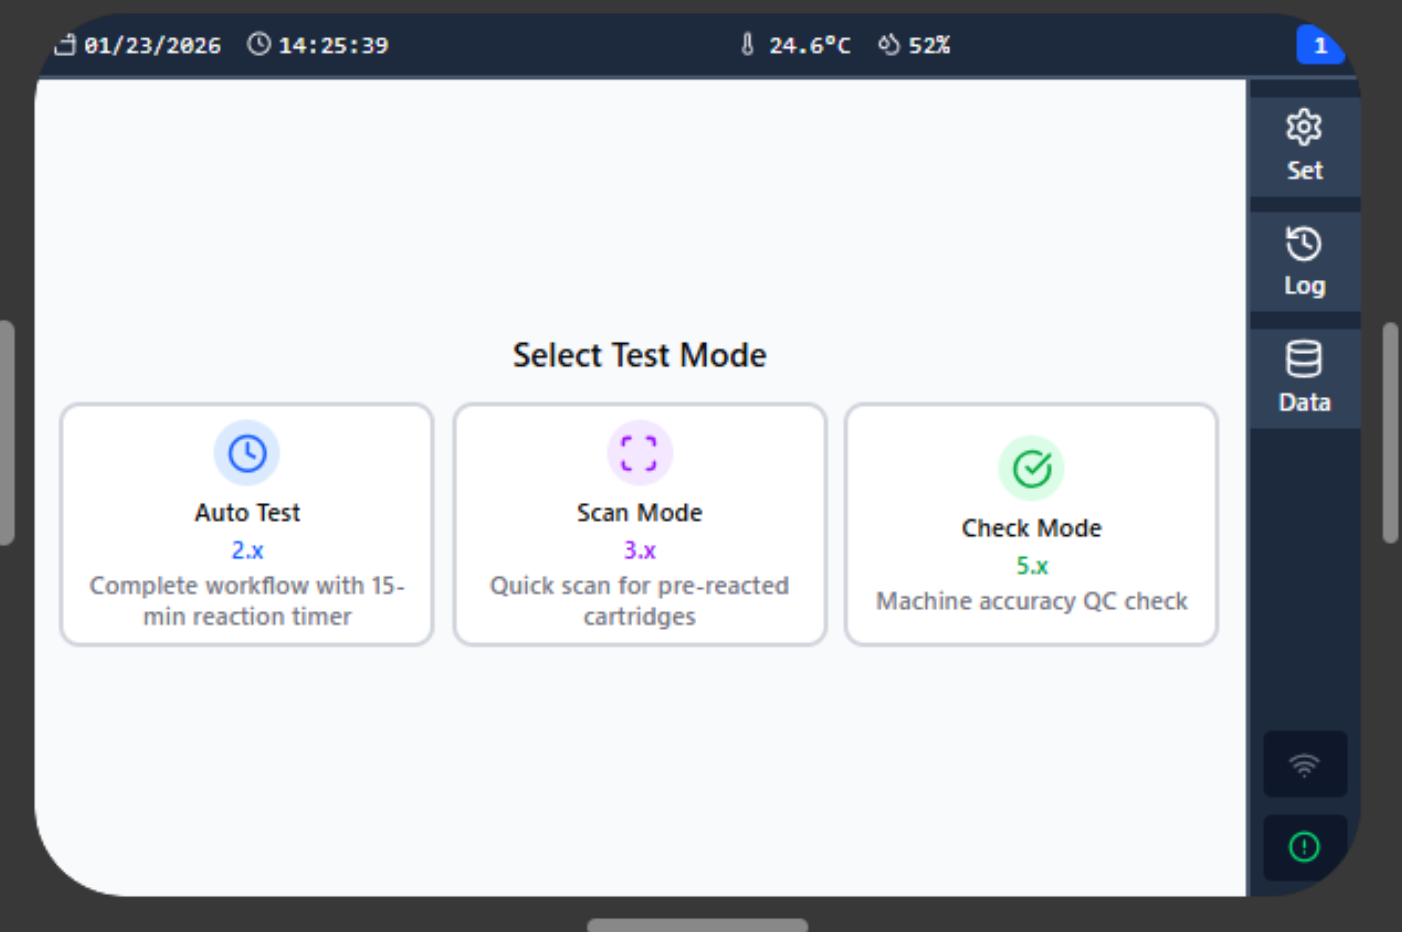
\includegraphics[width=\linewidth,height=3.5cm,keepaspectratio]{pic/12-1.png}
        \end{center}
        \vspace{0.4em}
        \begin{itemize}\setlength\itemsep{0.25em}
          \item \textbf{状態管理:} React Hooks（useState）
          \item \textbf{描画:} ブラウザDOMレンダリング
          \item \textbf{特徴:} 動的な要素配置とCSS装飾
        \end{itemize}
      \end{block}
    \end{column}
    \begin{column}{0.49\textwidth}
      \begin{block}{LVGL Implementation}
        \textbf{組み込み向け（C++17/Absolute）の堅牢なレイアウト。}
        \vspace{0.4em}
        \begin{center}
          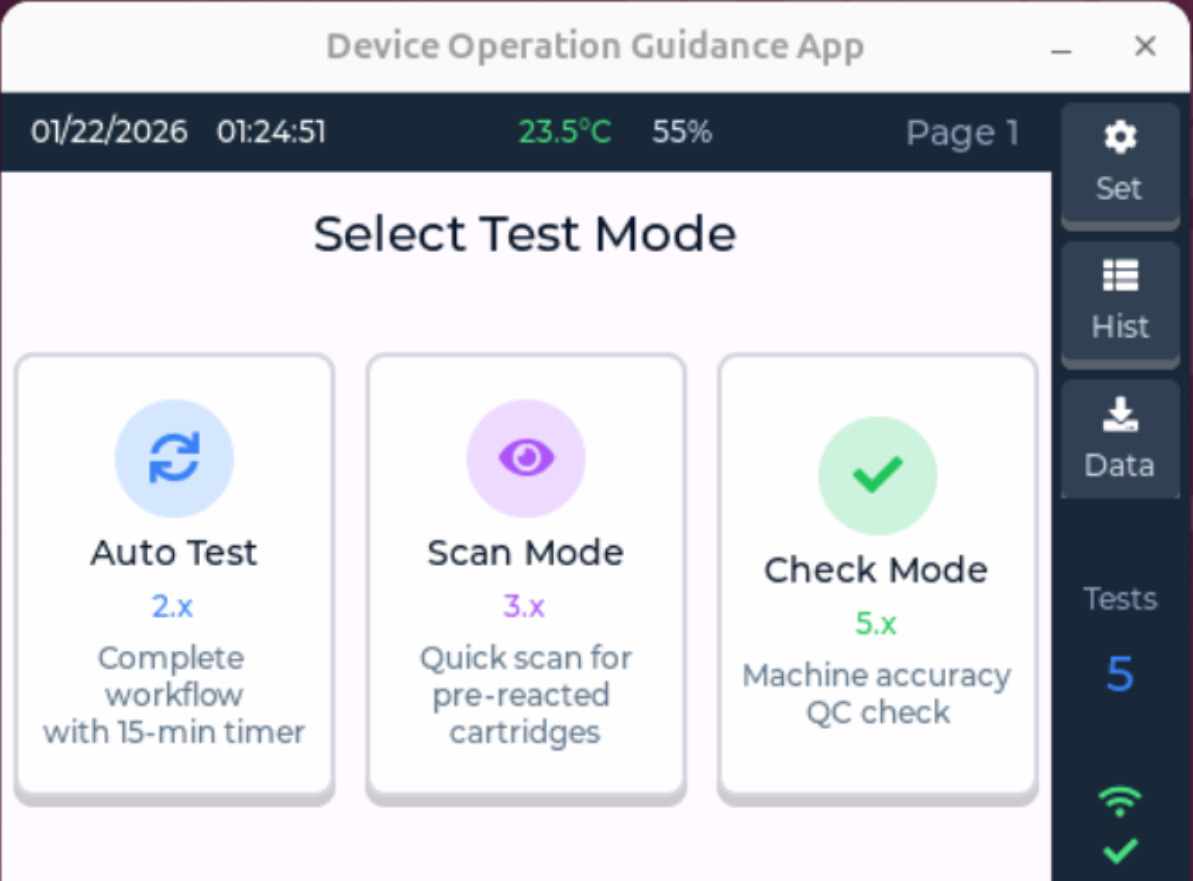
\includegraphics[width=\linewidth,height=3.5cm,keepaspectratio]{pic/12-2.png}
        \end{center}
        \vspace{0.4em}
        \begin{itemize}\setlength\itemsep{0.25em}
          \item \textbf{状態管理:} StateMachineクラス（C++）
          \item \textbf{描画:} フレームバッファへの直接描画
          \item \textbf{特徴:} 固定ピクセル配置とメモリ管理（RAII）
        \end{itemize}
      \end{block}
    \end{column}
  \end{columns}
\end{frame}

\section{フェーズ3}
\begin{frame}[t]{フェーズ3：Cursor・Copilotとの対話・デバッグ}
  \begin{block}{曖昧な指示からの意図理解と解決}
    自然言語によるフィードバックから、具体的なコード修正案を導き出す。
  \end{block}

  \scriptsize
  \definecolor{cardred}{RGB}{255,244,244}
  \definecolor{cardblue}{RGB}{242,248,255}
  \setlength{\fboxsep}{0.5pt}
  \setlength{\fboxrule}{0.8pt}
  \setlength{\columnsep}{0.15cm}

  \begin{columns}[T,onlytextwidth]
    \begin{column}{0.49\textwidth}
      \fcolorbox{black!12}{cardred}{%
        \parbox[t][1.3cm][t]{\linewidth}{%
          \textbf{\textcolor{red!70!black}{\normalsize 「メニューの位置とサイズがおかしい」}}\\[0.25em]
          \vspace{0.4em}
          ドックと重ならないように、一番上側に移動し、トップにして%
        }%
      }
    \end{column}
    \begin{column}{0.49\textwidth}
      \fcolorbox{black!12}{cardblue}{%
        \parbox[t][1.3cm][t]{\linewidth}{%
          \textbf{\textcolor{tsinghua}{\normalsize 座標計算による精密配置}}\\[0.25em]
          ステータスバー直下かつドックの左隣（$x=150,\ y=10$）へピクセル単位で再配置し、独立したドロワーとして実装。%
        }%
      }
    \end{column}
  \end{columns}

  \vspace{0.4cm}

  \begin{columns}[T,onlytextwidth]
    \begin{column}{0.49\textwidth}
      \fcolorbox{black!12}{cardred}{%
        \parbox[t][1.3cm][t]{\linewidth}{%
          \textbf{\textcolor{red!70!black}{\normalsize 「ボタンが見切れていて押せない」}}\\[0.25em]
          画面下部のレイアウト崩れ。内容量をコントロールし、ボタンの位置を固定する%
        }%
      }
    \end{column}
    \begin{column}{0.49\textwidth}
      \fcolorbox{black!12}{cardblue}{%
        \parbox[t][1.3cm][t]{\linewidth}{%
          \textbf{\textcolor{tsinghua}{\normalsize 固定表示内容に絶対配置への切り替え}}\\[0.25em]
          Flexレイアウトの自動調整を廃止し、$480\times320$の解像度に合わせて全要素のサイズと位置を固定化。カード高さを200pxに圧縮しボタンエリアを確保。%
        }%
      }
    \end{column}
  \end{columns}

  \vspace{0.4cm}

  \begin{columns}[T,onlytextwidth]
    \begin{column}{0.49\textwidth}
      \fcolorbox{black!12}{cardred}{%
        \parbox[t][1.3cm][t]{\linewidth}{%
          % ★修正: 「表示されなく」→「表示されず」
          \textbf{\textcolor{red!70!black}{\normalsize 「機能の欠落と不具合」}}\\[0.25em]
          ボタンを押してもオーバーレイが表示されず、ワーニングポップアップを押しても反応しない%
        }%
      }
    \end{column}
    \begin{column}{0.49\textwidth}
      \fcolorbox{black!12}{cardblue}{%
        \parbox[t][1.3cm][t]{\linewidth}{%
          \textbf{\textcolor{tsinghua}{\normalsize 状態の管理修正}}\\[0.25em]
          親コンテナ（overlayContainer）がデフォルトで非表示だったことを特定。Application.cppを修正し、子要素だけでなく親コンテナの可視性も制御するように変更。%
        }%
      }
    \end{column}
  \end{columns}
\end{frame}

\section{結論}
\begin{frame}[t]{AI UI設計 vs 従来チーム開発：効率比較}
  \small
  \begin{block}{開発アプローチの比較分析}
    \setlength{\tabcolsep}{7pt}
    \renewcommand{\arraystretch}{1.6}
    \rowcolors{2}{white}{black!2}
    % ★修正: 「数人　」の全角スペースを削除
    \begin{tabular}{>{\raggedright\arraybackslash}p{0.2\linewidth} >{\centering\arraybackslash}p{0.2\linewidth} >{\centering\arraybackslash}p{0.2\linewidth} >{\centering\arraybackslash}p{0.2\linewidth}}
      \rowcolor{tsinghua!15}
      \textbf{比較項目} & \textbf{AI支援（現行）} & \textbf{従来チーム} & \textbf{効率化}\tabularnewline
      \textbf{チーム構成} & 1名 + AI & 数人 & \textcolor{red!80!black}{人数大幅減}\tabularnewline
      \textbf{UI設計期間} & 最短1週 & 数週間 & \textcolor{red!80!black}{数倍短縮}\tabularnewline
      \textbf{コード実装} & 数週間 & 数ヶ月 & \textcolor{red!80!black}{数倍短縮}\tabularnewline
      \textbf{修正・調整} & 即時対応 & 会議調整 & \textcolor{red!80!black}{大幅改善}\tabularnewline
      \textbf{コスト} & 低 & 高 & \textcolor{red!80!black}{大幅削減}\tabularnewline
      \rowcolor{green!10}
      \textbf{総期間} & \textcolor{blue!70!black}{約数週間} & \textcolor{red!70!black}{約数ヶ月} & \textcolor{green!40!black}{数倍短縮}\tabularnewline
    \end{tabular}

    \vspace{0.6em}
    \fcolorbox{orange!70!black}{orange!10}{\parbox{0.96\linewidth}{\centering\textbf{結論:} 開発期間\textcolor{red!80!black}{数倍短縮}、コスト\textcolor{red!80!black}{大幅削減}}}
  \end{block}
\end{frame}


\begin{frame}[t]{結論}
  \large
  \centering
  AI Agentによる開発プロセスの変革\\[0.8em]

  \normalsize
  設計、環境構築、実装、修正の全フェーズにおいて\\
  AIエージェントが「エンジニアのペア」として機能\\[1.0em]

  \begin{columns}[T,onlytextwidth]
    \begin{column}{0.48\textwidth}
      \begin{block}{達成事項}
        \small
        \begin{itemize}\setlength\itemsep{0.25em}
          \item ReactからC++17への完全移行
          \item VMネットワーク環境の自動構築
          \item オフライン開発フローの確立
        \end{itemize}
      \end{block}
    \end{column}
    \begin{column}{0.48\textwidth}
      \begin{block}{今後の展望}
        \small
        \begin{itemize}\setlength\itemsep{0.25em}
          \item ハードウェア連携（駆動、センサーなどの実装）
          \item 仕様確定に伴うUI画面と操作の再調整
          \item 実機LCDテストへの展開と調整
        \end{itemize}
      \end{block}
    \end{column}
  \end{columns}
\end{frame}

\section{Appendix}
\begin{frame}[t]{A.1. LVGLのPro機能について}
  \begin{center}
    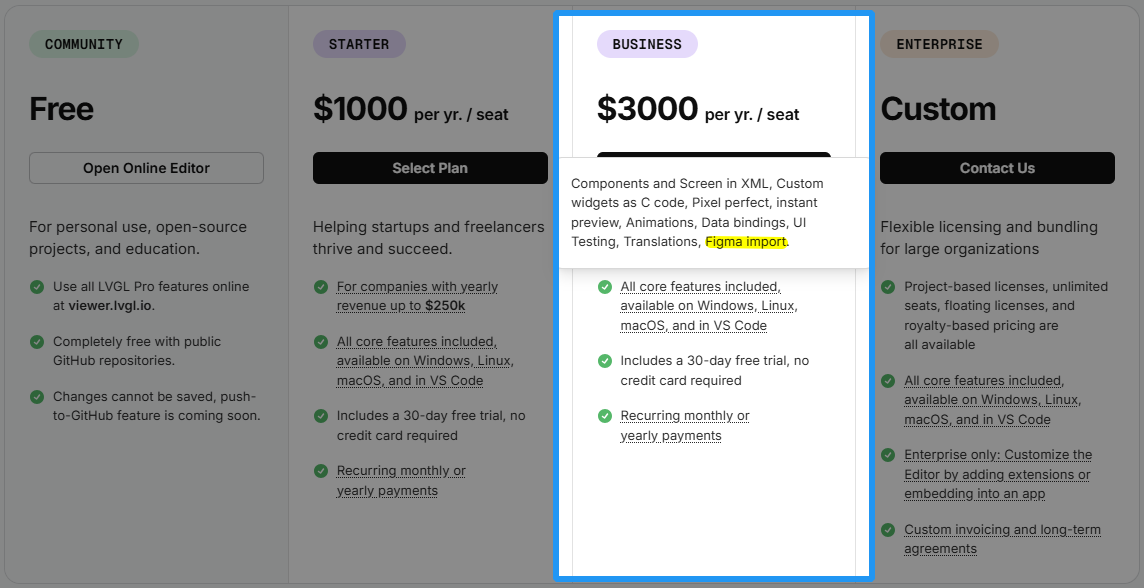
\includegraphics[width=\linewidth,height=0.72\textheight,keepaspectratio]{pic/A1_2.png}
  \end{center}

  \vspace{-0.5em}
  {\scriptsize 参考：\texttt{pro.lvgl.io/pricing}}
\end{frame}

\begin{frame}[t]{A.2. 標準測定の時UIの様子}
  \begin{center}
    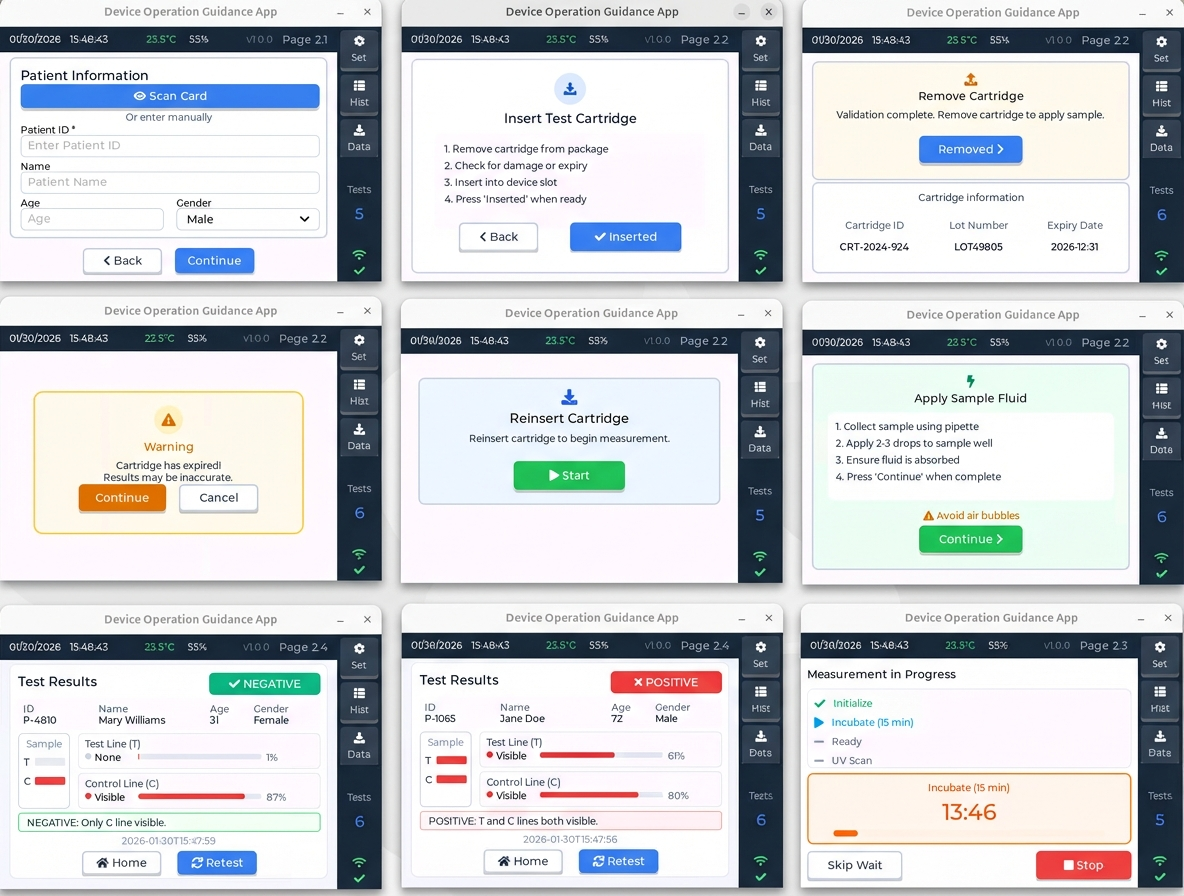
\includegraphics[width=\linewidth,height=0.8\textheight,keepaspectratio]{pic/A2_2.png}
  \end{center}
\end{frame}

\end{document}
